\section{State of The Art}

Reinforcement Learning is about use observed rewards to learn an optimal (or nearly optimal) 
policy for the environment \cite{russell2002artificial}. In other words, it is maximizing an 
agent's reward by performing a series of actions in response to a dynamic environment.

\begin{figure}[ht]
    \centering
    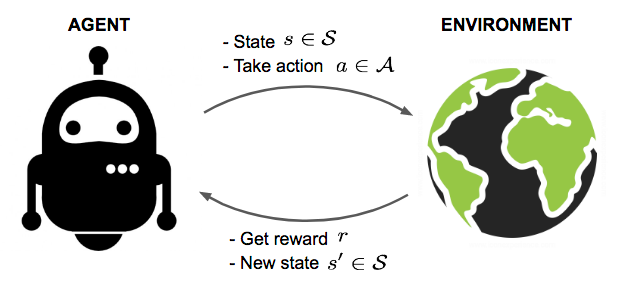
\includegraphics[scale=0.4]{images/RL_illustration.png}
    \caption{Simple diagram of the functioning of an RL system.}
    \label{fig:RL_illustration}
\end{figure}

After papers like "Playing Atari with Deep Reinforcement Learning"\cite{mnih2013playing} and "Reward is enough"\cite{silver2021reward} the enthusiasm for the RL has risen more and more. 

"Playing Atari with Deep Reinforcement Learning" presents the first deep learning model to successfully learn control policies directly from high-dimensional sensory inputs (raw pixels) using Reinforcement Learning \cite{mnih2013playing}.

"Reward is enough" hypothesizes how intelligence can be understood as subservient to reward maximization. The reward is enough to drive behavior that displays skills studied in natural and artificial intelligence. This is in contrast to the idea that specialized problem formulations, based on other signals or goals, are required for each skill \cite{silver2021reward}.

